\documentclass[tikz, border=5mm, ]{standalone}

% --------------------------------------------------
% Csomagok és könyvtárak
% --------------------------------------------------
\usepackage{tikz}
\usetikzlibrary{math} % matematikai számítások Tikz-ben
\usetikzlibrary{calc} % geometriai számítások (pl. koordináták)
\usetikzlibrary{angles} % szögjelölések rajzolása
\usetikzlibrary{quotes} % címkék és feliratok egyszerű kezelése
\usetikzlibrary{arrows.meta} % nyílstílusok
\usetikzlibrary{decorations.markings} % díszítések

% --------------------------------------------------
% mechTikz stílusok és parancsok
% --------------------------------------------------
%%%%%%%%%%%%%%%%%%%%%%%%%%%%%%%%%%%%%%%%%%%%%%%%%%%%
% mechTikz - Rúd szerkezetek rajzolása TikZ segítségével
%%%%%%%%%%%%%%%%%%%%%%%%%%%%%%%%%%%%%%%%%%%%%%%%%%%%

% --------------------------------------------------
% Alapstílusok
% --------------------------------------------------
% Definiáljuk a gyakran használt TikZ stílusokat
% (pl. pontok, rudak, erővektorok, stb.)

\tikzset{
  point/.style = {circle,fill=black,inner sep = 1.5pt},
  link/.style = {color=#1, very thick},
  angle/.style={color=#1,<->, >=latex},
  vec/.style = {color=#1,very thick,-latex},
  arc vec/.style={color=#1,very thick, postaction={decorate}, decoration={markings,mark=at position 1 with {\arrow{>}}}},
  arc vec2/.style={color=#1,very thick, postaction={decorate}, decoration={markings,mark=at position 1 with {\arrow{<}}}},
  force/.style = {color=#1, very thick,-latex},
  moment/.style = {color=#1,very thick,-Implies, double distance=1pt},
  coordSys/.style = {color=#1, thin,-latex},
  guide/.style = {color=#1,thin},
  guideVec/.style = {color=#1,latex-latex},
  construct/.style = {color=#1,thick,dashed},
  support/.style={link={black}, fill=white}
}

%%%%%%%%%%%%%%%%%%%%%%%%%%%%%%%%%%%%%%%%%%%%%%%%%%%%
% Saját TikZ parancsok definiálása
%%%%%%%%%%%%%%%%%%%%%%%%%%%%%%%%%%%%%%%%%%%%%%%%%%%%
% Ezek a parancsok új "rajzelemeket" hoznak létre, 
% amiket később egyszerűen, rövid paranccsal hívhatunk 
% meg rajzolás közben (pl. \supporthinge{A}{0}).

% --------------------------------------------------
% Általános elemek
% --------------------------------------------------

% Távolságjelölő makró
\newcommand{\dimarrow}[7][]{%
  % #1: opcionális TikZ stílus (pl. color=red, thick, stb.)
  % #2: első pont
  % #3: második pont
  % #4: eltolás vektor 1 (pl. (0,-1.25) vagy (1,0))
  % #5: eltolás vektor 2 (pl. (0,-1.25) vagy (1,0))
  % #6: felirat a nyíl közepén
  % #7: felirat pozíció (pl. below, above, left, right)
  \begin{scope}[#1]
    % vezető vonalak
    \draw[guide={gray}] ($(#2)+#4$) -- (#2);
    \draw[guide={gray}] ($(#3)+#5$) -- (#3);
    % távolság nyíl felirattal
    \draw[guideVec={gray}] ($(#2)+#4$) -- node[midway, #7] {#6} ($(#3)+#5$);
  \end{scope}
}

% Kis koordinátarendszer megrajzolása
\newcommand{\coordSys}[2][]{%
  % #1: opcionális paraméter (pl. scale=1.2, draw=blue, stb.)
  % #2: csomópont koordinátája (pl. (2,3))
  \begin{scope}[shift={(#2)}, #1]
    % x tengely
    \draw[coordSys={red}] (-0.5,0) -- (0.5,0) node[right] {$x$};
    % y tengely
    \draw[coordSys={red}] (0,-0.5) -- (0,0.5) node[above] {$y$};
  \end{scope}
}

% --------------------------------------------------
% Mechanikai elemek
% --------------------------------------------------

% Csuklós alátámasztás + ground
\newcommand{\supporthinge}[3][]{%
  % #1: opcionális paraméter (pl. scale=1.2, draw=blue, stb.)
  % #2: csomópont koordinátája
  % #3: forgatási szög fokban
  \begin{scope}[shift={(#2)}, rotate=#3, #1]
    % Talaj
    \fill[gray!20!white] (-0.5,-0.5) rectangle (0.5,-0.75);
    \draw[black, very thick] (-0.5,-0.5) -- (0.5,-0.5);
    % Háromszög
    \draw[support] (0,0) -- (-0.25,-0.5) -- (0.25,-0.5) -- cycle;
    \fill[white, draw={black}] (0,0) circle (0.1cm);
  \end{scope}
}

% Görgős alátámasztás + ground
\newcommand{\supportroller}[3][]{%
  % #1: opcionális paraméter
  % #2: csomópont koordinátája
  % #3: forgatási szög fokban
  \begin{scope}[shift={(#2)}, rotate=#3, #1]
    % Talaj
    \fill[gray!20!white] (-0.5,-0.5) rectangle (0.5,-0.75);
    \draw[black, very thick] (-0.5,-0.5) -- (0.5,-0.5);
    % Háromszög + görgők
    \draw[support] (0,0) -- (-0.25,-0.35) -- (0.25,-0.35) -- cycle;
    \foreach \i in {-0.15,0,0.15} {
      \draw[support] (\i,-0.425) circle (0.075);
    }
    \fill[white, draw={black}] (0,0) circle (0.1cm);
  \end{scope}
}

% Befogás
\newcommand{\supportfixed}[3][]{%
  % #1: opcionális paraméter (pl. line width, color, stb.)
  % #2: csomópont koordinátája
  % #3: forgatási szög fokban
  \begin{scope}[shift={(#2)}, rotate=#3, #1]
    % Talaj (befogás jelölés)
    \fill[gray!20!white] (-0.5,0) rectangle (0.5,-0.5);
    \draw[black, very thick] (-0.5,0) -- (0.5,0);
  \end{scope}
}

% Csúszka
\newcommand{\supportslider}[4][]{%
  % #1: opcionális paraméter (pl. line width, color, stb.)
  % #2: csomópont koordinátája
  % #3: forgatási szög fokban
  % #4: sín szélessége (alapértelmezett: 1)
  \begin{scope}[shift={(#2)}, rotate=#3, #1]
    % Felső sín
    \fill[gray!20!white] (-0.75,#4/2) rectangle (0.75,#4/2+0.25);
    \draw[black, very thick] (-0.75,#4/2) -- (0.75,#4/2);
    % Alsó sín
    \fill[gray!20!white] (-0.75,-#4/2) rectangle (0.75,-#4/2-0.25);
    \draw[black, very thick] (-0.75,-#4/2) -- (0.75,-#4/2);
  \end{scope}
}

% Kötél kényszer
\newcommand{\supportrope}[4][]{%
  % #1: opcionális paraméter (pl. scale, color, stb.)
  % #2: csomópont koordinátája
  % #3: forgatási szög fokban (pl. ha nem függőleges kábelt akarsz)
  \begin{scope}[shift={(#2)}, rotate=#3, #1]
    % Talaj (felfogatási pont)
    \fill[gray!20!white] (-0.5,-#4-0.25) rectangle (0.5,-#4-0.5);
    \draw[black, very thick] (-0.5,-#4-0.25) -- (0.5,-#4-0.25); 
    % Kötél
    \draw[black, thick, densely dashed] (0,0) -- (0,-#4-0.25);
    % Pontok
    \fill[black] (0,-#4-0.25) circle (0.05); % alsó pont
    \fill[black] (0,0) circle (0.05);        % felső pont
  \end{scope}
}

% Sima támasz + ground
\newcommand{\supportsimple}[3][]{%
  % #1: opcionális paraméter (pl. scale=1.2, draw=blue, stb.)
  % #2: csomópont koordinátája
  % #3: forgatási szög fokban
  \begin{scope}[shift={(#2)}, rotate=#3, #1]
    % Talaj
    \fill[gray!20!white] (-0.5,-0.5) rectangle (0.5,-0.75);
    \draw[black, very thick] (-0.5,-0.5) -- (0.5,-0.5);
    % Félkör támasz
    \draw[support] (0.25,-0.25) arc[start angle=0, end angle=180, radius=0.25];
    % Oldalsó vonalak a félkörhöz
    \draw[support] (-0.25,-0.25) -- (-0.25,-0.5) (0.25,-0.5) -- (0.25,-0.25) -- cycle;
  \end{scope}
}

% Csukló
\newcommand{\hinge}[2][]{%
  % #1: opcionális paraméter (pl. scale=1.2, draw=blue, stb.)
  % #2: csomópont koordinátája
  \begin{scope}[shift={(#2)}, #1]
    \fill[white, draw={black}] (0,0) circle (0.1cm);
  \end{scope}
}

% --------------------------------------------------
% Dokumentum kezdete
% --------------------------------------------------
\begin{document}

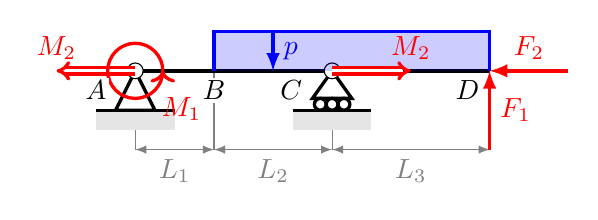
\begin{tikzpicture}

    \def\a{1}
    \def\b{1.5}
    \def\c{2}

    % Coordinates
    \coordinate (A) at (0,0);
    \coordinate (B) at (\a,0);
    \coordinate (C) at (\a+\b,0);
    \coordinate (D) at (\a+\b+\c,0);

    % Guides
    \dimarrow{A}{B}{(0,-1)}{(0,-1)}{$L_1$}{below}
    \dimarrow{B}{C}{(0,-1)}{(0,-1)}{$L_2$}{below}
    \dimarrow{C}{D}{(0,-1)}{(0,-1)}{$L_3$}{below}
    
    % Body
    \draw[link={black}] (A) -- (B) -- (C) -- (D);

    % Constraints
    \supporthinge{A}{0}
    \supportroller{C}{0}

    % Loads
    \draw[link={blue}, fill={blue}, fill opacity=0.2] (B) -- ($(B)+(0,0.5)$) -- ($(D)+(0,0.5)$) -- (D);
    \draw[force={blue}] ($(C)+(-0.75,0.5)$) -- ($(C)+(-0.75,0)$) node[midway, right] {$p$};
    \draw[force={red}] ($(D)+(1,0)$) -- (D) node[midway, above] {$F_2$};
    \draw[force={red}] ($(D)+(0,-1)$) -- (D) node[midway, right] {$F_1$};
    \draw[moment={red}] (C) -- ($(C)+(1,0)$) node[at end, above] {$M_2$};
    \draw[moment={red}] (A) -- ($(A)+(-1,0)$) node[at end, above] {$M_2$};
    \draw[arc vec={red}] (A) circle[radius=0.35] node[below right=0.2cm] {$M_1$};
  
    % Labels
    \node[below=0.25em, xshift=-0.5cm, fill=white, inner sep=1pt] at (A) {$A$};
    \node[below=0.25em, fill=white, inner sep=1pt] at (B) {$B$};
    \node[below left=0.25em, xshift=-0.25cm, fill=white, inner sep=1pt] at (C) {$C$};
    \node[below left=0.25em, fill=white, inner sep=1pt] at (D) {$D$};

\end{tikzpicture}
%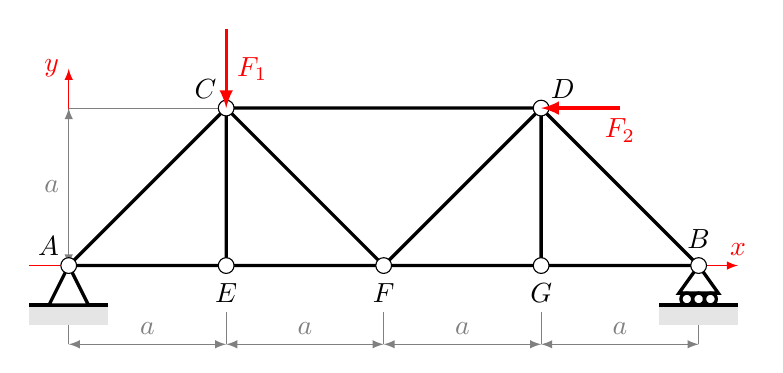
\begin{tikzpicture}

    \def\a{2}

    % Coordinates
    \coordinate (A) at (0,0);
    \coordinate (B) at (4*\a,0);
    \coordinate (C) at (\a,\a);
    \coordinate (D) at (3*\a,\a);
    \coordinate (E) at (\a,0);
    \coordinate (F) at (2*\a,0);
    \coordinate (G) at (3*\a,0);

    %Coordinate system
    \draw[coordSys={red}] ($(A)+(-0.5,0)$) -- ($(A)+(4*\a+0.5,0)$) node[above] {$x$};
    \draw[coordSys={red}] ($(A)+(0,-0.5)$) -- ($(A)+(0,\a+0.5)$) node[left] {$y$};

    % Guides
    \dimarrow{A}{E}{(0,-1)}{(0,-1)}{$a$}{above}
    \dimarrow{E}{F}{(0,-1)}{(0,-1)}{$a$}{above}
    \dimarrow{F}{G}{(0,-1)}{(0,-1)}{$a$}{above}
    \dimarrow{G}{B}{(0,-1)}{(0,-1)}{$a$}{above}
    \dimarrow{A}{C}{(0, 0)}{(-\a,0)}{$a$}{left}
    
    % Body
    \draw[link={black}] (A) -- (E) -- (F) -- (G) -- (B) -- (D) -- (C) -- cycle;
    \draw[link={black}] (E) -- (C) -- (F);
    \draw[link={black}] (F) -- (D) -- (G);

    % Constraints
    \supporthinge{A}{0}
    \supportroller{B}{0}
    \foreach \point in {C,D,E,F,G} {
        \hinge{\point}
    }

    % Loads
    \draw[vec={red}] ($(C)+(0,1)$) -- (C) node[midway, right] {$F_1$};
    \draw[vec={red}] ($(D)+(1,0)$) -- (D) node[at start, below] {$F_2$};
    
    % Labels
    \node[above left] at (A) {$A$};
    \node[above=0.25em] at (B) {$B$};
    \node[above left] at (C) {$C$};
    \node[above right] at (D) {$D$};
    \node[below=0.3em, fill=white] at (E) {$E$};
    \node[below=0.3em, fill=white] at (F) {$F$};
    \node[below=0.3em, fill=white] at (G) {$G$};

\end{tikzpicture}
%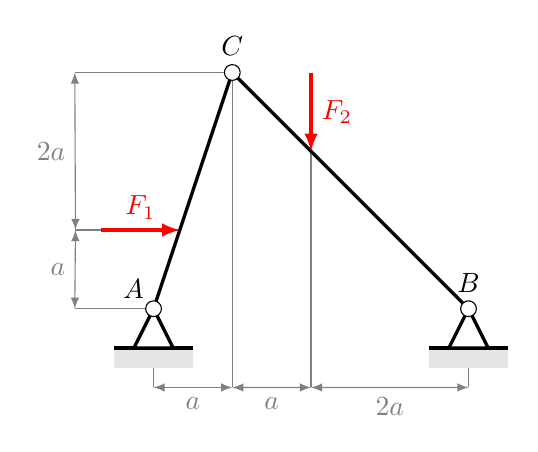
\begin{tikzpicture}

    \def\a{1}

    % Coordinates
    \coordinate (A) at (0,0);
    \coordinate (B) at (4*\a,0);
    \coordinate (C) at (\a,3*\a);
    \coordinate (F1) at ($2/3*(A)+1/3*(C)$);
    \coordinate (F2) at ($2/3*(C)+1/3*(B)$);

    %Coordinate system
    %\draw[coordSys={red}] ($(A)+(-0.5,0)$) -- ($(A)+(4*\a+1,0)$) node[above] {$x$};
    %\draw[coordSys={red}] ($(A)+(0,-0.5)$) -- ($(A)+(0,\a+0.5)$) node[left] {$y$};

    % Guides
    \dimarrow{A}{C}{(0,-1)}{(0,-3*\a-1)}{$a$}{below}
    \dimarrow{C}{F2}{(0,-3*\a-1)}{(0,-3*\a)}{$a$}{below}
    \dimarrow{F2}{B}{(0,-3*\a)}{(0,-1)}{$2a$}{below}

    \dimarrow{A}{F1}{(-1,0)}{(-\a-0.325,0)}{$a$}{left}
    \dimarrow{F1}{C}{(-\a-0.325,0)}{(-2,0)}{$2a$}{left}
    
    % Body
    \draw[link={black}] (A) -- (C) -- (B);

    % Constraints
    \supporthinge{A}{0}
    \supporthinge{B}{0}
    \hinge{C}

    % Loads
    \draw[vec={red}] ($(F1)+(-1,0)$) -- (F1) node[midway, above] {$F_1$};
    \draw[vec={red}] ($(F2)+(0,1)$) -- (F2) node[midway, right] {$F_2$};

    % Labels
    \node[above left] at (A) {$A$};
    \node[above=0.25em] at (B) {$B$};
    \node[above=0.25em] at (C) {$C$};

\end{tikzpicture}
%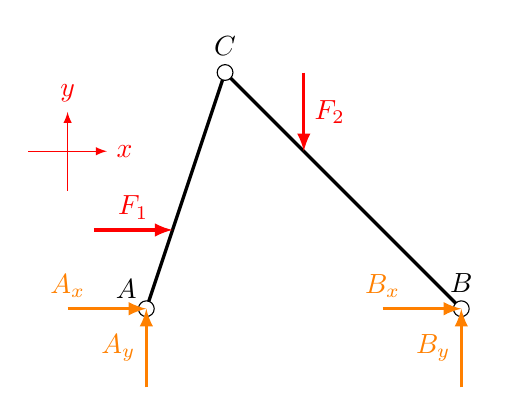
\begin{tikzpicture}

    \def\a{1}

    % Coordinates
    \coordinate (A) at (0,0);
    \coordinate (B) at (4*\a,0);
    \coordinate (C) at (\a,3*\a);
    \coordinate (F1) at ($2/3*(A)+1/3*(C)$);
    \coordinate (F2) at ($2/3*(C)+1/3*(B)$);

    %Coordinate system
    \coordSys{-1,2}
    
    % Body
    \draw[link={black}] (A) -- (C) -- (B);

    % Constraints
    \hinge{A}
    \hinge{B}
    \hinge{C}

    % Loads
    \draw[vec={red}] ($(F1)+(-1,0)$) -- (F1) node[midway, above] {$F_1$};
    \draw[vec={red}] ($(F2)+(0,1)$) -- (F2) node[midway, right] {$F_2$};

    % Reaction forces
    \draw[vec={orange}] ($(A)+(-1,0)$) -- (A) node[at start, above] {$A_x$};
    \draw[vec={orange}] ($(A)+(0,-1)$) -- (A) node[midway, left] {$A_y$};
    \draw[vec={orange}] ($(B)+(-1,0)$) -- (B) node[at start, above] {$B_x$};
    \draw[vec={orange}] ($(B)+(0,-1)$) -- (B) node[midway, left] {$B_y$};

    % Labels
    \node[above left] at (A) {$A$};
    \node[above=0.25em] at (B) {$B$};
    \node[above=0.25em] at (C) {$C$};

\end{tikzpicture}
%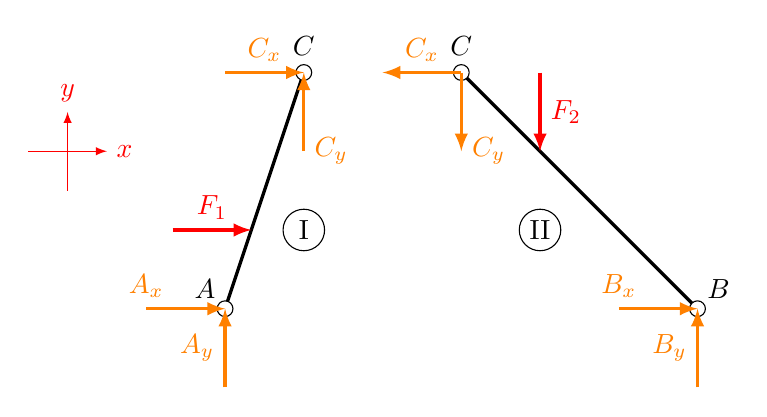
\begin{tikzpicture}
    \def\a{1}

    %==== AC member ====
    \begin{scope}
        % Coordinates
        \coordinate (A) at (0,0);
        \coordinate (C) at (\a,3*\a);

        %Coordinate system
        \coordSys{-2,2}

        % Body
        \draw[link={black}] (A) -- (C);

        % Constraints
        \hinge{A}
        \hinge{C}

        % Loads
        \coordinate (F1) at ($2/3*(A)+1/3*(C)$);
        \draw[vec={red}] ($(F1)+(-1,0)$) -- (F1) node[midway, above] {$F_1$};

        % Reaction forces
        \draw[vec={orange}] ($(A)+(-1,0)$) -- (A) node[at start, above] {$A_x$};
        \draw[vec={orange}] ($(A)+(0,-1)$) -- (A) node[midway, left] {$A_y$};
        \draw[vec={orange}] ($(C)+(0,-1)$) -- (C) node[at start, right] {$C_y$};
        \draw[vec={orange}] ($(C)+(-1,0)$) -- (C) node[midway, above] {$C_x$};

        % Labels
        \node[above left] at (A) {$A$};
        \node[above=0.25em] at (C) {$C$};
        \node[circle, draw=black, inner sep=0pt,minimum size=1.5em] at (\a,\a) {I};
    \end{scope}

    %==== CB member (shifted) ====
    \begin{scope}[xshift=2cm]
        % Coordinates
        \coordinate (C) at (\a,3*\a);
        \coordinate (B) at (4*\a,0);

        % Body
        \draw[link={black}] (C) -- (B);

        % Constraints
        \hinge{C}
        \hinge{B}

        % Loads
        \coordinate (F2) at ($2/3*(C)+1/3*(B)$);
        \draw[vec={red}] ($(F2)+(0,1)$) -- (F2) node[midway, right] {$F_2$};

        % Reaction forces
        \draw[vec={orange}] ($(B)+(-1,0)$) -- (B) node[at start, above] {$B_x$};
        \draw[vec={orange}] ($(B)+(0,-1)$) -- (B) node[midway, left] {$B_y$};
        \draw[vec={orange}] (C) -- ($(C)+(0,-1)$) node[at end, right] {$C_y$};
        \draw[vec={orange}] (C) -- ($(C)+(-1,0)$) node[midway, above] {$C_x$};

        % Labels
        \node[above right] at (B) {$B$};
        \node[above=0.25em] at (C) {$C$};
        \node[circle, draw=black, inner sep=0pt,minimum size=1.5em] at (2*\a,\a) {II};
    \end{scope}

\end{tikzpicture}


\end{document}
